% Common preamble for PIGMIE patent figures (A4).
% Drawing conventions:
%   - A4 portrait
%   - Sans-serif throughout (Helvetica)
%   - "Fig. N" sentence-case caption near top
%   - Page "N/total" at top centre
%   - Reference numerals outside boxes via leader lines
%   - ALL CAPS labels in component boxes
%   - Reactor uses north-east-lines hatched fill
%   - Scene uses double-line border
%   - Module enclosures use dashed line with internal numeral

\documentclass[a4paper,10pt]{article}
\usepackage[top=2.5cm,bottom=1.0cm,left=2.5cm,right=1.5cm]{geometry}
\usepackage[T1]{fontenc}
\usepackage{helvet}
\renewcommand{\familydefault}{\sfdefault}
\usepackage{amsmath,amssymb,bm}
\usepackage{tikz}
\usetikzlibrary{shapes,shapes.geometric,shapes.misc,arrows.meta,positioning,fit,calc,backgrounds,decorations.pathreplacing,decorations.markings,patterns}
\pagestyle{empty}
\setlength{\parindent}{0pt}

\tikzset{
  % Component box: ALL CAPS label inside, no numeral inside
  cbox/.style={draw, rectangle, minimum height=1.0cm, minimum width=2.4cm,
               align=center, line width=0.5pt, font=\small},
  cbox-tall/.style={cbox, minimum height=1.6cm},
  cbox-wide/.style={cbox, minimum width=3.0cm},
  cbox-narrow/.style={cbox, minimum width=1.8cm, font=\footnotesize},
  % Reactor / physical medium: hatched fill
  reactor/.style={cbox, pattern=north east lines, pattern color=black!70},
  % Scene: double-line border
  scenebox/.style={cbox, double, double distance=1.2pt, line width=0.4pt},
  % Module / sub-module enclosure
  enclosure/.style={draw, rectangle, dashed, line width=0.4pt, inner sep=10pt, rounded corners=2pt},
  enclosure-solid/.style={draw, rectangle, line width=0.5pt, inner sep=10pt, rounded corners=2pt},
  % Arrows
  flowarr/.style={-Latex, line width=0.5pt, font=\scriptsize},
  flowbi/.style={Latex-Latex, line width=0.5pt, font=\scriptsize},
  flowarr-fb/.style={-Latex, line width=0.5pt, dashed, font=\scriptsize},
  % Reference numeral leader-line endpoint and label
  refnum/.style={font=\footnotesize, inner sep=1pt},
  leader/.style={line width=0.4pt, -Latex},
  % Caption banner
  figcap/.style={font=\bfseries\large}
}

% Helper: figure header (page number + Fig. N caption)
\newcommand{\figheader}[3]{%
  % #1 = page number (e.g. "1"), #2 = total pages, #3 = figure label (e.g. "1" or "4A")
  \noindent\hfill\small #1/#2\hfill\null\par
  \vspace{0.2cm}
  \begin{center}\bfseries Fig.\ #3\end{center}
  \vspace{0.2cm}
}


\begin{document}

\figheader{6}{7}{5}

\begin{center}
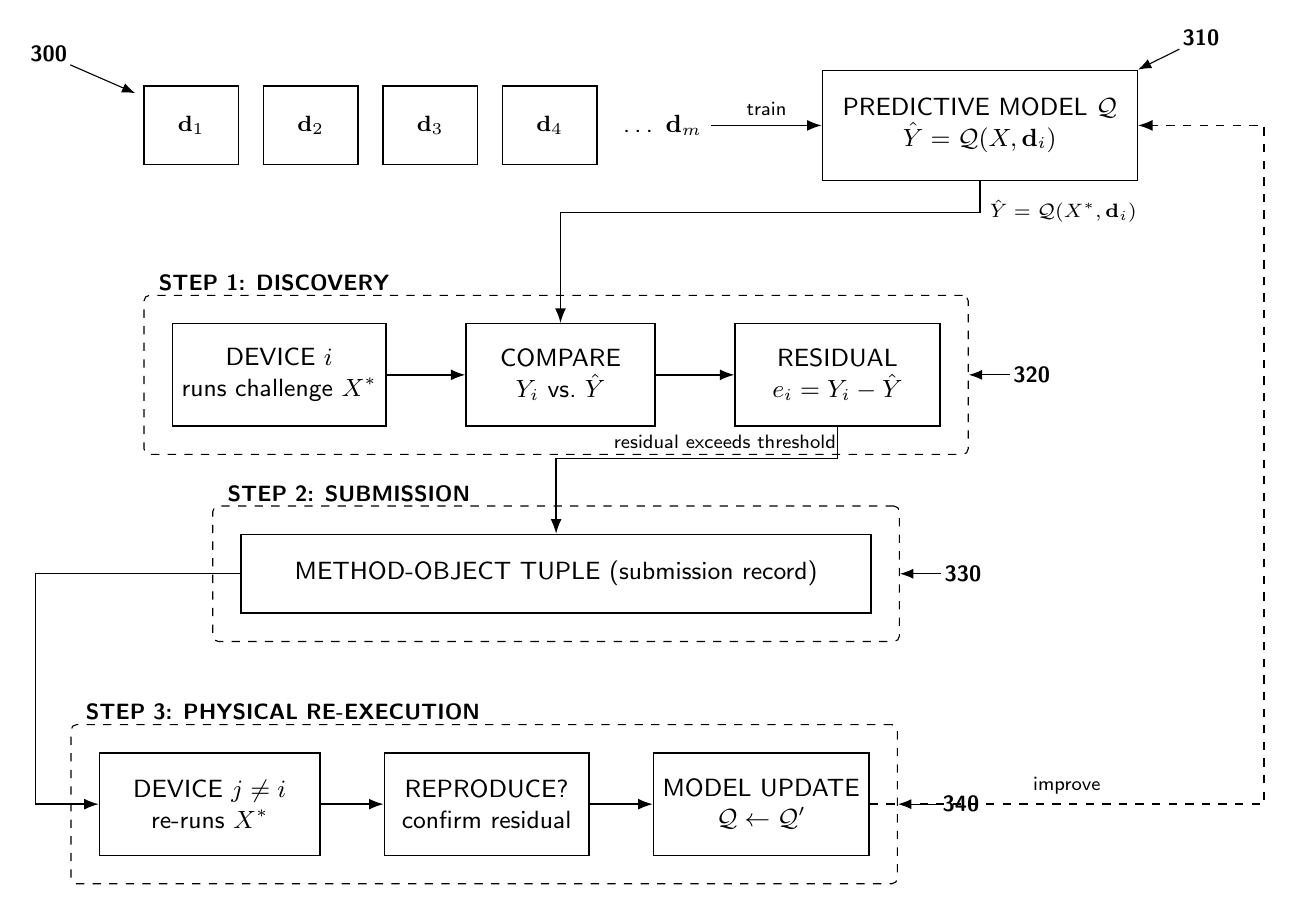
\begin{tikzpicture}[node distance=8mm]

% ============== Top: fleet device representations 300, training -> predictive model 310 ==============
\node[cbox-narrow, minimum width=1.2cm] (d1) {$\mathbf{d}_1$};
\node[cbox-narrow, right=3mm of d1, minimum width=1.2cm] (d2) {$\mathbf{d}_2$};
\node[cbox-narrow, right=3mm of d2, minimum width=1.2cm] (d3) {$\mathbf{d}_3$};
\node[cbox-narrow, right=3mm of d3, minimum width=1.2cm] (d4) {$\mathbf{d}_4$};
\node[anchor=west, font=\small] at ($(d4.east)+(2mm,0)$) (dots) {\ldots\ $\mathbf{d}_m$};

\node[cbox-wide, right=14mm of dots, minimum width=4.0cm, minimum height=1.4cm] (model)
  {PREDICTIVE MODEL $\mathcal{Q}$\\$\hat{Y} = \mathcal{Q}(X,\mathbf{d}_i)$};

\draw[flowarr] (dots.east) -- node[above, font=\scriptsize] {train} (model.west);

% ============== STEP 1: DISCOVERY (320) ==============
\node[cbox, below=20mm of d2, xshift=-4mm, minimum width=2.6cm, minimum height=1.3cm] (s1dev) {DEVICE $i$\\runs challenge $X^{*}$};
\node[cbox, right=10mm of s1dev, minimum width=2.4cm, minimum height=1.3cm] (s1cmp) {COMPARE\\$Y_i$ vs.\ $\hat{Y}$};
\node[cbox, right=10mm of s1cmp, minimum width=2.6cm, minimum height=1.3cm] (s1res) {RESIDUAL\\$e_i = Y_i - \hat{Y}$};

\draw[flowarr] (s1dev.east) -- (s1cmp.west);
\draw[flowarr] (s1cmp.east) -- (s1res.west);

% Predictive model output feeds COMPARE
% Route: model.south -> down -> left into s1cmp.north; label below model south, clear of train arrow
\draw[flowarr] (model.south) -- ++(0,-4mm)
  node[pos=0.95, right, font=\scriptsize] {$\hat{Y}=\mathcal{Q}(X^{*},\mathbf{d}_i)$}
  -| (s1cmp.north);

\begin{scope}[on background layer]
  \node[enclosure, fit=(s1dev)(s1cmp)(s1res), inner sep=10pt] (step1) {};
\end{scope}
\node[font=\footnotesize\bfseries, anchor=south west] at ($(step1.north west)+(2pt,-2pt)$) {STEP 1: DISCOVERY};

% ============== STEP 2: SUBMISSION (330) ==============
\node[cbox-wide, below=10mm of step1.south, minimum width=8cm, minimum height=1.0cm] (s2)
  {METHOD-OBJECT TUPLE (submission record)};

\begin{scope}[on background layer]
  \node[enclosure, fit=(s2), inner sep=10pt] (step2) {};
\end{scope}
\node[font=\footnotesize\bfseries, anchor=south west] at ($(step2.north west)+(2pt,-2pt)$) {STEP 2: SUBMISSION};

% ============== STEP 3: PHYSICAL RE-EXECUTION (340) ==============
\node[cbox, below=14mm of step2.south, xshift=-44mm, minimum width=2.8cm, minimum height=1.3cm] (s3dev) {DEVICE $j \neq i$\\re-runs $X^{*}$};
\node[cbox, right=8mm of s3dev, minimum width=2.6cm, minimum height=1.3cm] (s3rep) {REPRODUCE?\\confirm residual};
\node[cbox, right=8mm of s3rep, minimum width=2.6cm, minimum height=1.3cm] (s3upd) {MODEL UPDATE\\$\mathcal{Q} \leftarrow \mathcal{Q}'$};

\draw[flowarr] (s3dev.east) -- (s3rep.west);
\draw[flowarr] (s3rep.east) -- (s3upd.west);

\begin{scope}[on background layer]
  \node[enclosure, fit=(s3dev)(s3rep)(s3upd), inner sep=10pt] (step3) {};
\end{scope}
\node[font=\footnotesize\bfseries, anchor=south west] at ($(step3.north west)+(2pt,-2pt)$) {STEP 3: PHYSICAL RE-EXECUTION};

% ============== Step-to-step arrows ==============
% s1res -> s2 (residual exceeds threshold -> submission)
\draw[flowarr] (s1res.south) -- ++(0,-4mm) -| node[pos=0.2, above, font=\scriptsize] {residual exceeds threshold} (s2.north);

% s2 -> s3dev — endpoint at DEVICE j; arrowhead points east into s3dev.west
% Vertical descent column must be LEFT of s3dev.west so final segment runs west-to-east into the box
\coordinate (s3devCol) at ($(s3dev.west)+(-8mm,0)$);
\draw[flowarr] (s2.west) -- (s3devCol |- s2.west)
  -- (s3devCol |- s3dev.west)
  -- (s3dev.west);

% Feedback: step 3 model update -> back to predictive model 310 ("improve")
% Routed FAR OUTSIDE all step enclosures and the tuple table.
% improveCol must be RIGHT of model.east so the final segment enters the model from the east side
% (arrowhead at model.east correctly points west into the box)
\coordinate (improveCol) at ($(model.east)+(16mm,0)$);
\draw[flowarr-fb] (s3upd.east) -- (improveCol |- s3upd.east)
  node[pos=0.5, above, font=\scriptsize] {improve}
  -- (improveCol |- model.east)
  -- (model.east);

% ============== Reference numerals via leader lines ==============
% 300 (fleet representations) — top-left
\node[refnum] at ($(d1.north west)+(-12mm,4mm)$) (n300) {\textbf{300}};
\draw[leader] (n300.south east) -- ($(d1.north west)+(-1mm,-1mm)$);
% 310 (predictive model) — top-right
\node[refnum] at ($(model.north east)+(8mm,4mm)$) (n310) {\textbf{310}};
\draw[leader] (n310.south west) -- (model.north east);
% 320 (discovery step) — right of step1 enclosure
\node[refnum] at ($(step1.east)+(8mm,0)$) (n320) {\textbf{320}};
\draw[leader] (n320.west) -- (step1.east);
% 330 (submission) — right of step2 enclosure
\node[refnum] at ($(step2.east)+(8mm,0)$) (n330) {\textbf{330}};
\draw[leader] (n330.west) -- (step2.east);
% 340 (re-execution) — right of step3 enclosure
\node[refnum] at ($(step3.east)+(8mm,0)$) (n340) {\textbf{340}};
\draw[leader] (n340.west) -- (step3.east);

\end{tikzpicture}
\end{center}

\end{document}
